\chapter{Metodologia}

Przeprowadzenie tego badania sprowadzać się będzie do dwóch głównych metodologicznych aspektów: pozyskanie danych oraz sama analiza.

\section{Pozyskanie danych}

Dane są dostępne w~repozytorium baz danych UCI \cite{Dua:2021}, jednak dostęp programistyczny niezbędny przy zbieraniu tak dużych ilości danych jest utrudniony ze względu na brak API.
W takim wypadku trzeba posłużyć się starszym i~toporniejszym, ale bardziej uniwersalnym \emph{scraperem}.

\subsection{API (Application Programming Interface)}

Poprzez termin \emph{interfejs programowania aplikacji} (API) definiuje się interfejs pozwalający na bezpośrednią komunikację i~interakcję między serwisami czy programami.
Ludzie korzystają z~internetu w~sposób, który dla komputera jest niepotrzebnym skomplikowaniem -- istotna jest otoczka wizualna, intuicyjność i~prostota w~obsłudze, które z~kolei programowi utrudniają uzyskanie czystych danych.
Dlatego definiuje się osobne interfejsy, które pozwalają zewnętrznym serwisom na prostą, szybką i~bezpieczną interakcję, a~które nazywamy API.
Taki koncept pozwala na pisanie oprogramowań w~sposób modularny.
Szybkość, prostota i~bezpieczeństwo takiego podejścia dają ogromne możliwości, jeśli jest odpowiednio dobrze udokumentowana \cite{meng2018application}.

Szczególnie popularnym typem API, który można nawet określić standardem serwisów internetowych, jest \emph{REST} (inaczej nazywane \emph{RESTful API}), czyli Representational State Transfer.
Serwis oferujący dostęp standard REST udostępnia informacje tekstowo i~pozwala na ich czytanie i~zapisywanie przy pomocy predefiniowanych operacji i~protokołu bezstanowego, czyli niezależnie od sesji.
Gdy zaczęto używać określenie ``Web 2.0'' na sieć, która nie oferuje wyłącznie statycznych zasobów, ale składa się z~interaktywnych, wzajemnie połączonych serwisów, zauważono potencjał metodologii opartych na REST jako idealnego mechanizmu wiązania publikowanych danych semantycznych z~istniejącą architekturą sieci \cite{battle2008bridging}.
Tim O'Reilly zdefiniował w~tym temacie trzy główne aspekty \cite{o2009web}:
\begin{enumerate}
	\item \emph{Wsparcie lekkich modeli programowania, które pozwalają na luźno powiązane systemy}.
	W niektórych przypadkach ścisłe powiązanie serwisów jest niezbędne, jednak przy tworzeniu takowego z~myślą o~jego ogólnej dostępności, luźny dostęp jest istotniejszy nawet za cenę bezpieczeństwa.
	\item \emph{Myślenie o~syndykacji\footnotemark, nie koordynacji}.
	Proste serwisy internetowe powinny syndykować dane, nie próbując kontrolować co się z~nimi dzieje po drugiej stronie połączenia.
    \footnotetext{Syndykacja (sieciowa) to architektura bazująca na gromadzeniu przez klienta informacji z~wielu serwerów zewnętrznych, gdzie rolą serwera jest zebranie danych z~różnych źródeł. Przykładem technologii wykorzystującej syndykację jest RSS.}
	\item \emph{Projektowanie dla ``hackowalności'' oraz reużywalności}.
	Bariery reużywalności powinny być bardzo niskie.
\end{enumerate}

\subsection{Scraper}

Kiedy użycie publicznie dostępnego interfejsu API nie jest możliwe, jedyną alternatywą uzyskania dostępu do danych serwisu webowego jest starsza idea programu nazywanego ``skrobaczem'' -- \emph{scraper}.
Jest to prosty program, który uzyskuje dostęp do konkretnych danych poprzez wykorzystanie tego samego medium, z~którego korzystają ludzie czytając materiały w~sieci.
Najczęściej jest to więc dokument HTML, gdy weźmiemy pod uwagę najpopularniejszy typ \emph{scraperów}, czyli \emph{web scrapery}, służące do wyciągania danych ze stron internetowych.
Nie jest to rozwiązanie idealne, ponieważ zakłada potrzebę dostania się do informacji w~konkretnej części otrzymanego dokumentu, który jest zbiorem potężnej ilości znaczników, bardzo często niepowiązanych ze sobą.
Bardziej rozbudowane programy automatycznie przeszukują wszystkie podstrony z~danego zbioru linków i~pozwalają na wygenerowanie w~ten sposób zbioru danych w~formie tabelarycznej.
Implementacja takiego \emph{scrapera} składa się z~trzech części \cite{mahto2016dive}:
\begin{enumerate}
	\item Program typu \emph{pełzacz} (\emph{Web Crawler}), który wydobywa pożądane linki,
	\item Ekstraktor danych do wydobywania danych z~otrzymywanych linków,
	\item Zapisywanie wydobytych danych do pliku (na przykład \emph{.csv}).
\end{enumerate}
Wszystkie części implementacji można wykonać w~języku Python, który posiada wiele bibliotek znacznie ułatwiających ich wykonywanie.

Biblioteka \texttt{BeautifulSoup} jest kluczowym elementem \emph{scrapera}, jako że pozwala na idiomatyczną nawigację po dokumencie HTML.
Używa jednego z~podanych jej parserów (takich jak wbudowany w~standard języka \texttt{html.parser} lub bardzo szybki i~wydajny \texttt{lxml}) w~celu zbudowania drzewa znaczników dokumentu HTML zachowując wszystkie ich atrybuty.
Następnie przy pomocy tej biblioteki można swobodnie poruszać się po utworzonym drzewie wyszukując interesujące nas znaczniki o~podanych cechach, rekurencyjnie używając ich jako korzenia nowego drzewa wyszukiwań.

Przykładowe użycie biblioteki \texttt{BeautifulSoup} może wyglądać następująco:
\begin{lstlisting}[language=Python]
from bs4 import BeautifulSoup
from requests import get
site = get("https://example.com").text
soup = BeautifulSoup(site, features="lxml")
tab = soup.body.find_all("table")[1]
tab = tab.find_all("table", recursive=True)[3]
for tr in tab.find_all("tr", recursive=False)[1:]:
	...
\end{lstlisting}
Obiekt \texttt{BeautifulSoup} jest specjalną wersją obiektu \texttt{Tag}, która reprezentuje cały sparsowany dokument \cite{richardson2007beautiful}.
Za pomocą \lstinline{soup.body.find_all("table")[1]} odwołujemy się więc kolejno do znacznika \texttt{body} i~jego zawartości (w postaci obiektu klasy \texttt{Tag}),  tablicy wszystkich znaczników \texttt{table} znajdujących się wewnątrz ciała i~przypisujemy jej drugą wartość do nazwy \texttt{tab}.
W następnej linijce przeszukujemy znaleziony \texttt{Tag} w~celu odnalezienia znajdujących się w~nim kolejnych znaczników \texttt{table}.
Użycie parametru \lstinline{recursive=True}, mówi, że poszukiwanie zagnieżdżonych tabel powinno odbywać się w~obecnym znaczniku a~także rekursywnie w~każdym niżej.
W ten sposób odnajdujemy wszystkie tabele w~aktualnym znaczniku, wybieramy z~nich czwartą i~przypisujemy do nazwy \texttt{tab}.
Na koniec iterujemy po znacznikach \texttt{tr} wybranej tabeli omijając pierwszy z~nich zaznaczeniem, że interesują nas wyłącznie znaczniki na obecnym poziomie.

Takie rozwiązanie pozwala dostać się do dowolnych informacji zawartych na stronie internetowej, ale ma znaczącą wadę sprawiającą, że metoda ta powinna być używana wyłącznie przy braku innych możliwości.
Przeszukiwanie stron internetowych w~ten sposób jest oparte o~ich strukturę, często skomplikowaną i~z czasem zmienną.
Aby wiedzieć, gdzie znaleźć interesujące nas informacje musimy najpierw ręcznie przejrzeć źródło strony oraz jej strukturę, aby znaleźć ścieżkę prowadzącą do miejsca, w~którym oczekujemy znaleźć szukane dane.
Jeden znacznik, który pojawi się w~ramach błędu czy drobnych zmian na stronie może doprowadzić do zawieszenia działania \emph{scrapera}, lub spowoduje, że zacznie on zwracać niepoprawne dane, co jeszcze długo może pozostać niezauważone.
Działanie utrudnia sposób budowania stron internetowych (w szczególności w~nowszych technologiach), który z~oczywistych względów generuje bardzo skomplikowane i~złożone drzewa znacznikowe prowadząc do serwisów wizualnie przyjemniejszych, ale trudniejszych do nawigacji przez \emph{scrapery}.

\emph{Scraping} przy dostępności odpowiadającego mu API jest zdecydowanie gorszym rozwiązaniem, ale jego mocną stroną jest właśnie uniwersalność i~umożliwienie dotarcia do wszelkich danych na stronie.
Za pomocą tego rozwiązania można stworzyć systemy marketingowe potrafiące uzyskiwać kontekst informacji na generycznych stronach i~w ten sposób dobierać pasujące reklamy \cite{vargiu2013exploiting}.

Biblioteka \texttt{pandas} jest z~kolei szczególnie przydatna, gdy wymagane są jakieś operacje na zbiorze danych, takie jak wstępne przetworzenie wydobytych informacji.
Operuje ona na danych w~postaci tabelarycznej, składających się z~kolumn (atrybutów) oraz wierszy (rekordów).
Częste operacje w~ramach wstępnej obróbki to konwersja typów danych, usunięcie zbędnych czy błędnych rekordów lub dodanie nowych kolumn bazujących na pozostałych danych.
Przykładowo może być to zamienienie kolumny zawierającej datę publikacji na liczbę dni od publikacji, gdy taka informacja jest bardziej adekwatna.

\section{Analiza danych}

Największą wartość z~wydobytych danych można uzyskać dopiero, gdy przetworzy się je i~przeanalizuje.
Istnieje wiele sposobów na przeprowadzenie takiej analizy, z~których jednym jest użycie wspomnianej biblioteki \texttt{pandas}.
Dodatkowym atutem wyboru tego narzędzia jest możliwość ściślejszego powiązania części analizującej programu z~jego częścią wydobywającą dane.
Jednak użycie tej biblioteki nie jest idealnym rozwiązaniem, gdy głównym celem jest eksploracja uzyskanych danych, gdzie wykorzystanie narzędzi wizualnych jest bardziej optymalne.

\subsection{Microsoft Azure Machine Learning Studio}

\begin{figure}[ht]
	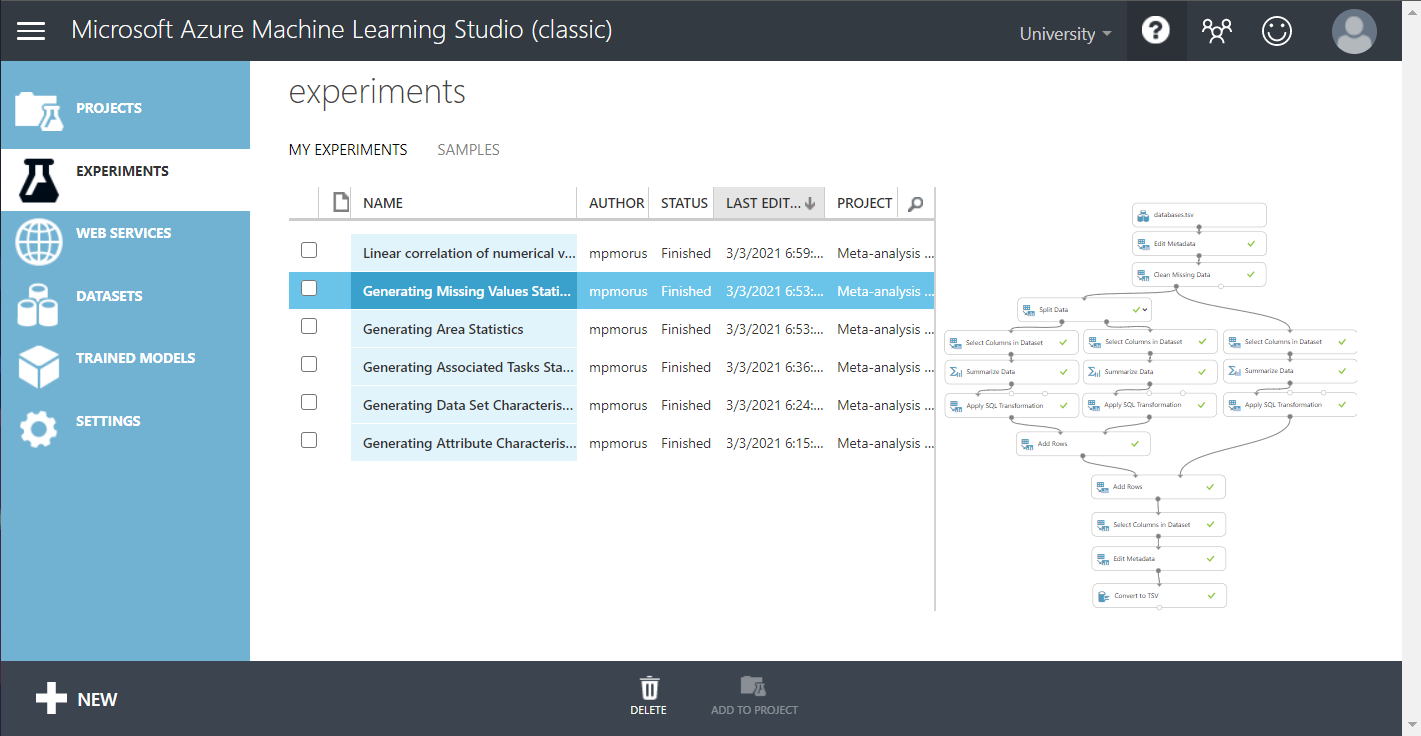
\includegraphics[width=\textwidth]{Screenshots/AzureML_interface}
	\caption{Interfejs programu Microsoft Azure Machine Learning Studio (classic)}
	\label{fig:interface}
\end{figure}

Microsoft Azure Machine Learning Studio (dalej \emph{Azure ML}) to platforma stworzona przez firmę Microsoft oferująca interaktywną, wizualną przestrzeń roboczą przeznaczoną do tworzenia, testowania i~wdrażania predykcyjnych modeli analitycznych.
Jest to aplikacja z~interfejsem webowym działająca w~przeglądarce (rysunek \ref{fig:interface}), na celu mająca tworzenie modeli uczenia maszynowego.
Mimo to sprawdza się znakomicie jako narzędzie do samej analizy, pozwalając na stopniową obróbkę danych oraz ich wizualizację i~przeglądanie na każdym kolejnym kroku.

Platforma oferuje możliwość importu i~eksportu \emph{zbiorów danych} do obszaru roboczego, w~którym pracujemy.
Podobnie można zapisywać i~zarządzać wytrenowanymi \emph{modelami} klasyfikatorów.
Tworzenie \emph{projektów} pozwala na organizację zapisanych zbiorów danych, modeli i~eksperymentów w~zbiory tematycznie ze sobą powiązane.
Te ostatnie są najistotniejszym elementem platformy, w~którym mieści się cała analiza danych, ich przetwarzanie i~trenowanie modeli.

\emph{Eksperyment} w~Azure ML to odrębny, kompletny obiekt przepływu informacji z~wbudowanymi wszystkimi komponentami potrzebnymi do tworzenia, testowania i~ewaluacji modeli predykcyjnych.
W eksperymencie moduły (komponenty) połączone są ze sobą liniami wskazującymi przepływ informacji i~parametrów z~wyjścia jednego do wejścia drugiego \cite{barga2015introducing}.

\begin{figure}[ht]
	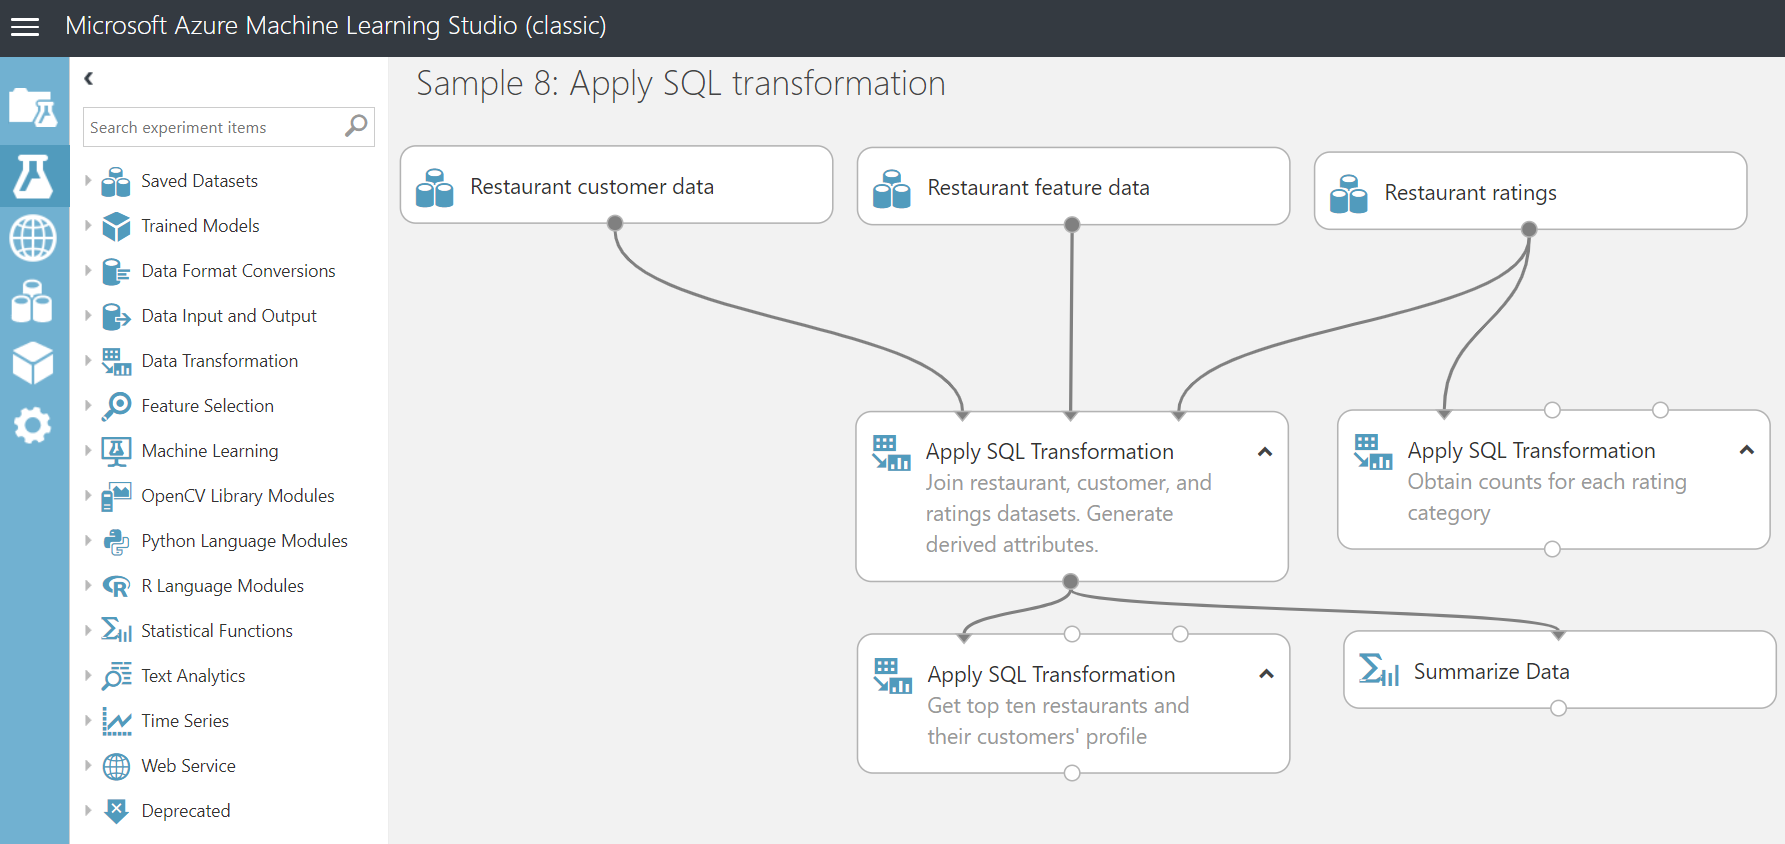
\includegraphics[width=\textwidth]{Screenshots/AzureML_experiment.png}
	\caption{Przykładowy schemat blokowy eksperymentu}
	\label{fig:experiment}
\end{figure}

Interfejs (rysunek \ref{fig:interface}) pozwala na intuicyjne, wizualne układanie i~łączenie odpowiednich bloków z~użyciem predefiniowanych modułów.
Modułu są kategoryzowane z~uwzględnieniem ich głównego przeznaczenia i~sposobu działania.
Można używać zbiorów danych zapisanych w~serwisie, przekształcać je i~modyfikować, wykorzystać i~uczyć modele uczenia maszynowego oraz wykonywać obliczenia statystyczne.
Poza modułami o~ściśle określonym działaniu dostępne są również bloki pozwalające na wykonaniu na zbiorze danych zdefiniowanego przez użytkownika skryptu SQL (jak na rysunku \ref{fig:experiment}), skryptu napisanego w~Pythonie oraz skryptu w~języku R.
Możliwość wykorzystania tych języków programowania w~przetwarzaniu danych sprawia, że Azure ML staje się bardzo potężnym narzędziem, gdzie w~razie potrzeby można zdefiniować niestandardowe i~bardzo skomplikowane sposoby przetworzenia danych, jednocześnie nie tracąc na łatwości i~intuicyjności wykonywania prostszych operacji za pomocą dostępnych modułów.

Dodatkowo Azure ML posiada dwa bloki specjalne, ``web service input'' oraz ``web service output'', które pozwalają na utworzenie na bazie wykonywanego eksperymentu serwisu webowego wykonywanego w~chmurze Azure.
Umożliwia to udostępnienie wykonywanej obróbki danych do wykonania we wszelkich projektach deweloperskich z~dostępem do internetu.
Dane wejściowe wysyła się jako dane zapytania na serwer pod otrzymanym adresem wraz z~kluczem API danego serwisu webowego, a~dane wyjściowe otrzymuje się jako odpowiedź serwera na to zapytanie.
